\documentclass[12pt,a4paper]{scrartcl}

\author{Rafael Dorigo, Sebastian Hirnschall}
%% (C) Hirnschall Sebastian, Rafael 2019
\date{\today}


\usepackage[
backend=biber,
style=authoryear-icomp,    % Zitierstil
isbn=false,                % ISBN nicht anzeigen, gleiches geht mit nahezu allen anderen Feldern
pagetracker=true,          % ebd. bei wiederholten Angaben (false=ausgeschaltet, page=Seite, spread=Doppelseite, true=automatisch)
maxbibnames=50,            % maximale Namen, die im Literaturverzeichnis angezeigt werden (ich wollte alle)
maxcitenames=3,            % maximale Namen, die im Text angezeigt werden, ab 4 wird u.a. nach den ersten Autor angezeigt
autocite=inline,           % regelt Aussehen für \autocite (inline=\parancite)
block=space,               % kleiner horizontaler Platz zwischen den Feldern
backref=true,              % Seiten anzeigen, auf denen die Referenz vorkommt
backrefstyle=three+,       % fasst Seiten zusammen, z.B. S. 2f, 6ff, 7-10
date=short                % Datumsformat
]{biblatex}

\addbibresource{./refs.bib}

\usepackage{longtable}
%\usepackage{hyperref}
\usepackage{amsmath}% http://ctan.org/pkg/amsmath
\usepackage[ngerman]{cleveref} %referenzen fur Abbildungen
\usepackage{graphicx}
\usepackage{listings}
\usepackage{esdiff}
\usepackage[utf8]{inputenc}
\usepackage[ngerman]{babel}
\usepackage[T1]{fontenc}
\usepackage{graphicx}
\usepackage{amssymb}
\usepackage{geometry}% http://ctan.org/pkg/geometry
\usepackage{amsthm}
\usepackage{tocloft}
\usepackage{framed}
\usepackage{mathtools}
\usepackage{color}
\usepackage{multirow}
\usepackage{textcomp}
\usepackage{float}
%\usepackage[dvipsnames]{xcolor}
\usepackage{mathtools}
\usepackage{caption}
\usepackage{subcaption}

%\usepackage[ruled,vlined]{algorithm2e}
\usepackage{algorithmicx}
\usepackage{algorithm}
\usepackage[noend]{algpseudocode}

\makeatletter
\def\BState{\State\hskip-\ALG@thistlm}
\makeatother

\usepackage[table,xcdraw,dvipsnames]{xcolor}

\usepackage{fancyvrb}


%\pagestyle{headings}

\setcounter{secnumdepth}{5}
\setcounter{tocdepth}{5}

%\pagestyle{headings}

\usepackage{fancyhdr}
\pagestyle{fancy}
%
\rhead{ }
%\rhead[re]{\textbf{\nouppercase{\leftmark}}}
\chead{}
\lhead{\leftmark}
%%
\lfoot{Rafael Dorigo, Sebastian Hirnschall}
\cfoot{}
\rfoot{\thepage}
%%
\renewcommand{\headrulewidth}{0.2pt}
\renewcommand{\footrulewidth}{0.2pt}
\newcommand{\R}{\mathbb{R}}


\fancypagestyle{general}
{
	\fancyhf{}
	\rhead{}
	%\rhead[re]{\textbf{\nouppercase{\leftmark}}}
	\chead{}
	\lhead{\leftmark}
	\lfoot{Rafael Dorigo, Sebastian Hirnschall}
	\cfoot{}
	\rfoot{\thepage}
}


%listings settings
\definecolor{mygreen}{rgb}{0,0.6,0}
\definecolor{mygray}{rgb}{0.5,0.5,0.5}
\definecolor{mymauve}{rgb}{0.58,0,0.82}
\definecolor{BackgroundGray}{rgb}{0.9,0.9,0.9}

\lstset{ %
	backgroundcolor=\color{BackgroundGray},   % choose the background color; you must add \usepackage{color} or \usepackage{xcolor}
	basicstyle=\footnotesize,        % the size of the fonts that are used for the code
	breakatwhitespace=false,         % sets if automatic breaks should only happen at whitespace
	breaklines=true,                 % sets automatic line breaking
	captionpos=b,                    % sets the caption-position to bottom
	commentstyle=\color{mygreen},    % comment style
	deletekeywords={...},            % if you want to delete keywords from the given language
	escapeinside={\%*}{*)},          % if you want to add LaTeX within your code
	extendedchars=true,              % lets you use non-ASCII characters; for 8-bits encodings only, does not work with UTF-8
	frame=single,	                   % adds a frame around the code
	keepspaces=true,                 % keeps spaces in text, useful for keeping indentation of code (possibly needs columns=flexible)
	keywordstyle=\color{blue},       % keyword style
	language=C,                 	   % the language of the code
	otherkeywords={*,...},           % if you want to add more keywords to the set
	numbers=left,                    % where to put the line-numbers; possible values are (none, left, right)
	numbersep=5pt,                   % how far the line-numbers are from the code
	numberstyle=\tiny\color{mygray}, % the style that is used for the line-numbers
	rulecolor=\color{mygray},         % if not set, the frame-color may be changed on line-breaks within not-black text (e.g. comments (green here))
	showspaces=false,                % show spaces everywhere adding particular underscores; it overrides 'showstringspaces'
	showstringspaces=false,          % underline spaces within strings only
	showtabs=false,                  % show tabs within strings adding particular underscores
	stepnumber=2,                    % the step between two line-numbers. If it's 1, each line will be numbered
	stringstyle=\color{mymauve},     % string literal style
	tabsize=2,	                   % sets default tabsize to 2 spaces
	title=\lstname,                   % show the filename of files included with \lstinputlisting; also try caption instead of title
	emph={int,unsigned,long,vector,char,string},
	emphstyle={\color{ForestGreen}}
}

\Crefname{lstlisting}{Listing}{Listing}


%italic quotes
\newenvironment{italicquotes}
{\begin{quote}\itshape}
	{\end{quote}}


%tableofcontents font
%\renewcommand{\cftchapfont}{\scshape}
\renewcommand{\cftsecfont}{\bfseries}
\addtokomafont{disposition}{\rmfamily}

\newcommand{\spar}{\par\vspace{10pt}\noindent}
\newcommand{\Mod}[1]{\ (\text{mod}\ #1)}


\usepackage{twoopt}
\newcommandtwoopt{\img}[4][0.5cm][0.7]{
	\begin{figure}[!h]
		\vspace{#1}
		\centering
		\includegraphics[width=#2\textwidth]{#3}
		\caption{#4} %\footnotemark}
		\label{fig:#3}
	\end{figure}
	%\footnotetext{#5}
}


\numberwithin{equation}{section} 
%\makeatletter
%\@addtoreset{equation}{section}
%\makeatother


%\newtheorem{theorem}{Theorem}[section]
%\newtheorem{lemma}[theorem]{Lemma}
%\newtheorem{proposition}[theorem]{Proposition}
%\newtheorem{corollary}[theorem]{Corollary}

\newcounter{myalgctr}

\newenvironment{mydef}{%      define a custom environment
	\par\noindent%         create a vertical offset to previous material
	\refstepcounter{myalgctr}% increment the environment's counter
	\textsc{\textbf{Definition} \themyalgctr}% or \textbf, \textit, ...
	\newline
}{\par\bigskip}  %          create a vertical offset to following material
\numberwithin{myalgctr}{section}

\crefname{myalgctr}{Definition}{Definitionen}

%theorem
\newcounter{mytheoremctr}

\newenvironment{mytheorem}{%      define a custom environment
	\refstepcounter{mylemmactr}% increment the environment's counter
	\refstepcounter{mykorollarctr}
	\refstepcounter{mybeispielctr}% increment the environment's counter
	\refstepcounter{mytheoremctr}
	\par \noindent%         create a vertical offset to previous material
	\textsc{\textbf{Satz} \themytheoremctr}% or \textbf, \textit, ...
	\newline\noindent
}{\par\bigskip}  %          create a vertical offset to following material
\numberwithin{mytheoremctr}{subsection}

\crefname{mytheoremctr}{Satz}{Satz}

%korollar
\newcounter{mykorollarctr}

\newenvironment{mykorollar}{%      define a custom environment
	\refstepcounter{mylemmactr}% increment the environment's counter
	\refstepcounter{mytheoremctr}
	\refstepcounter{mybeispielctr}% increment the environment's counter
	\refstepcounter{mykorollarctr}
	\par\noindent%         create a vertical offset to previous material
	\textsc{\textbf{Korollar} \themykorollarctr}% or \textbf, \textit, ...
	\newline\noindent
}{\par\bigskip}  %          create a vertical offset to following material
\numberwithin{mykorollarctr}{subsection}

\crefname{mykorollarctr}{Korollar}{Korollar}

%lemma
\newcounter{mylemmactr}

\newenvironment{mylemma}{%      define a custom environment
	\refstepcounter{mykorollarctr}
	\refstepcounter{mytheoremctr}
	\refstepcounter{mybeispielctr}% increment the environment's counter
	\refstepcounter{mylemmactr}% increment the environment's counter
	\par\noindent%         create a vertical offset to previous material
	\textsc{\textbf{Lemma} \themylemmactr}% or \textbf, \textit, ...
	\newline\noindent
}{\par\bigskip}  %          create a vertical offset to following material
\numberwithin{mylemmactr}{subsection}

\crefname{mylemmactr}{Lemma}{Lemma}

\newcounter{mybeispielctr}

%beispiel
\newenvironment{mybeispiel}{%      define a custom environment
	\refstepcounter{mykorollarctr}
	\refstepcounter{mytheoremctr}
	\refstepcounter{mylemmactr}% increment the environment's counter
	\refstepcounter{mybeispielctr}% increment the environment's counter
	\par\noindent%         create a vertical offset to previous material
	\textsc{\textbf{Beispiel} \themybeispielctr}% or \textbf, \textit, ...
	\newline\noindent
}{\par\bigskip}  %          create a vertical offset to following material
\numberwithin{mybeispielctr}{subsection}

\crefname{mybeispielctr}{Beispiel}{Beispiel}

\newenvironment{myproof}{%      define a custom environment
	\bigskip\noindent%         create a vertical offset to previous material
	\textsc{\textbf{\\Beweis\\}}% or \textbf, \textit, ...
	\indent
}{\qed\par\bigskip}  %          create a vertical offset to following material

\newenvironment{bemerkung}{%      define a custom environment
	\bigskip\noindent%         create a vertical offset to previous material
	\textsc{\textbf{\\Bemerkung.}}% or \textbf, \textit, ...
	\indent
}{\par\bigskip}  %          create a vertical offset to following material

\newcommand{\mpar}[1]{\paragraph*{#1}\mbox{}\par}
\newcommand\norm[1]{\left\lVert#1\right\rVert}
\DeclarePairedDelimiter{\abs}{\lvert}{\rvert}


\pagestyle{fancy}
\fancypagestyle{firststyle}
{
	\fancyhf{}
	\rhead{}
	%\rhead[re]{\textbf{\nouppercase{\leftmark}}}
	\chead{}
	\lhead{\leftmark}
	\lfoot{Rafael Dorigo, Sebastian Hirnschall}
	\cfoot{}
	\rfoot{\thepage}
}

\crefname{section}{Abschnitt}{Abschnitt}

\setlength\parindent{0pt}
\begin{document}
	\newgeometry{bottom=1cm,top=1cm,left=1cm,right=1cm}
	\begin{titlepage}
		\begin{flushleft}
				
\includegraphics[width=.4\linewidth]{tuwien.png}
		\end{flushleft}	
		\centering
		
		
		\vspace{5cm}
		{\huge\bfseries CG-Verfahren f\"ur \\dünn besetzte Matrizen\par}
		\vspace{2cm}
		{\Large\itshape Rafael Dorigo\\Sebastian Hirnschall\par}
		\vspace{1cm}
		{\large\itshape Betreut von:\\Markus Wess Dipl.-Ing.\par}
		\vspace{1cm}
		\begin{figure}[!h]
			\vspace{0cm}
			\centering
			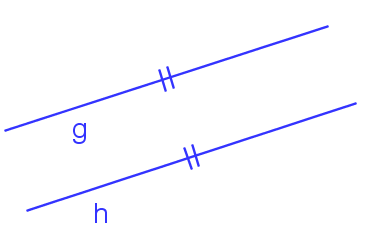
\includegraphics[width=.4\linewidth]{titelbild2.png}
		\end{figure}
		
		\vfill
		
		% Bottom of the page
		{\today\par}
	\end{titlepage}
	\restoregeometry
	
	\thispagestyle{firststyle}
	
	\newpage\noindent

	\thispagestyle{firststyle}
	
	\newpage
	\tableofcontents
	\thispagestyle{general}
	\newpage

	\section{Einleitung}
	Das Projekt beschäftigt sich mit dem Lösen linearer Gleichungssysteme der Form $Ax = b$. Dabei werden verschiedene iterative Verfahren vorgestellt und deren Aufwand verglichen. Außerdem wird eine effiziente Methode gezeigt, dünn besetzte Matrizen zu speichern. Es folgen Plots zur Veranschaulichung der Konvergenzgeschwindigkeit der Verfahren.
	\newpage
	
	\section{Aufwand einer symmetrisch positiv definiten Zufallsmatrix}
	Um für eine symmetrische positiv definite Koeffizientenmatrix $A\in\mathbb{R}^{n\times n}$ und $b \in \mathbb{R}^{n}$ die Gleichung $Ax = b$ zu lösen treten bei der Cholesky-Zerlegung $\frac{1}{3}n^{3} + \mathcal{O}(n^{2})$ arithmetische Operationen auf. \\
	Zum testen kann $A$ folgendermaßen Generiert werden. 
	
	
	\lstinputlisting[language=C++, firstline = 486, lastline= 509, caption = Erstellen einer symmertrisch postiv definiten Zufallsmatrix mit einer fixen Anzahl an Einträgen ungleich $0$ pro Zeile in C++]{../code/Linag/densematrix.h} 
	
	\begin{bemerkung}
		Die Implementierung aller Klassen und Funktionen im $linag$-namespace sind im Anhang zu finden. Zum Vergleich wurde die Eigen-Bibliothek verwendet. (\textit{http://eigen.tuxfamily.org}) 
	\end{bemerkung}
	
	Wie in \cref{fig:zeiteigensolver} zu sehen ist, ist das direkte Lösen bei großen Problemen nicht praktikabel, da die benötigte Zeit kubisch mit der Problemgröße steigt. 
	
	\begin{figure}[H]
		\begin{center}
			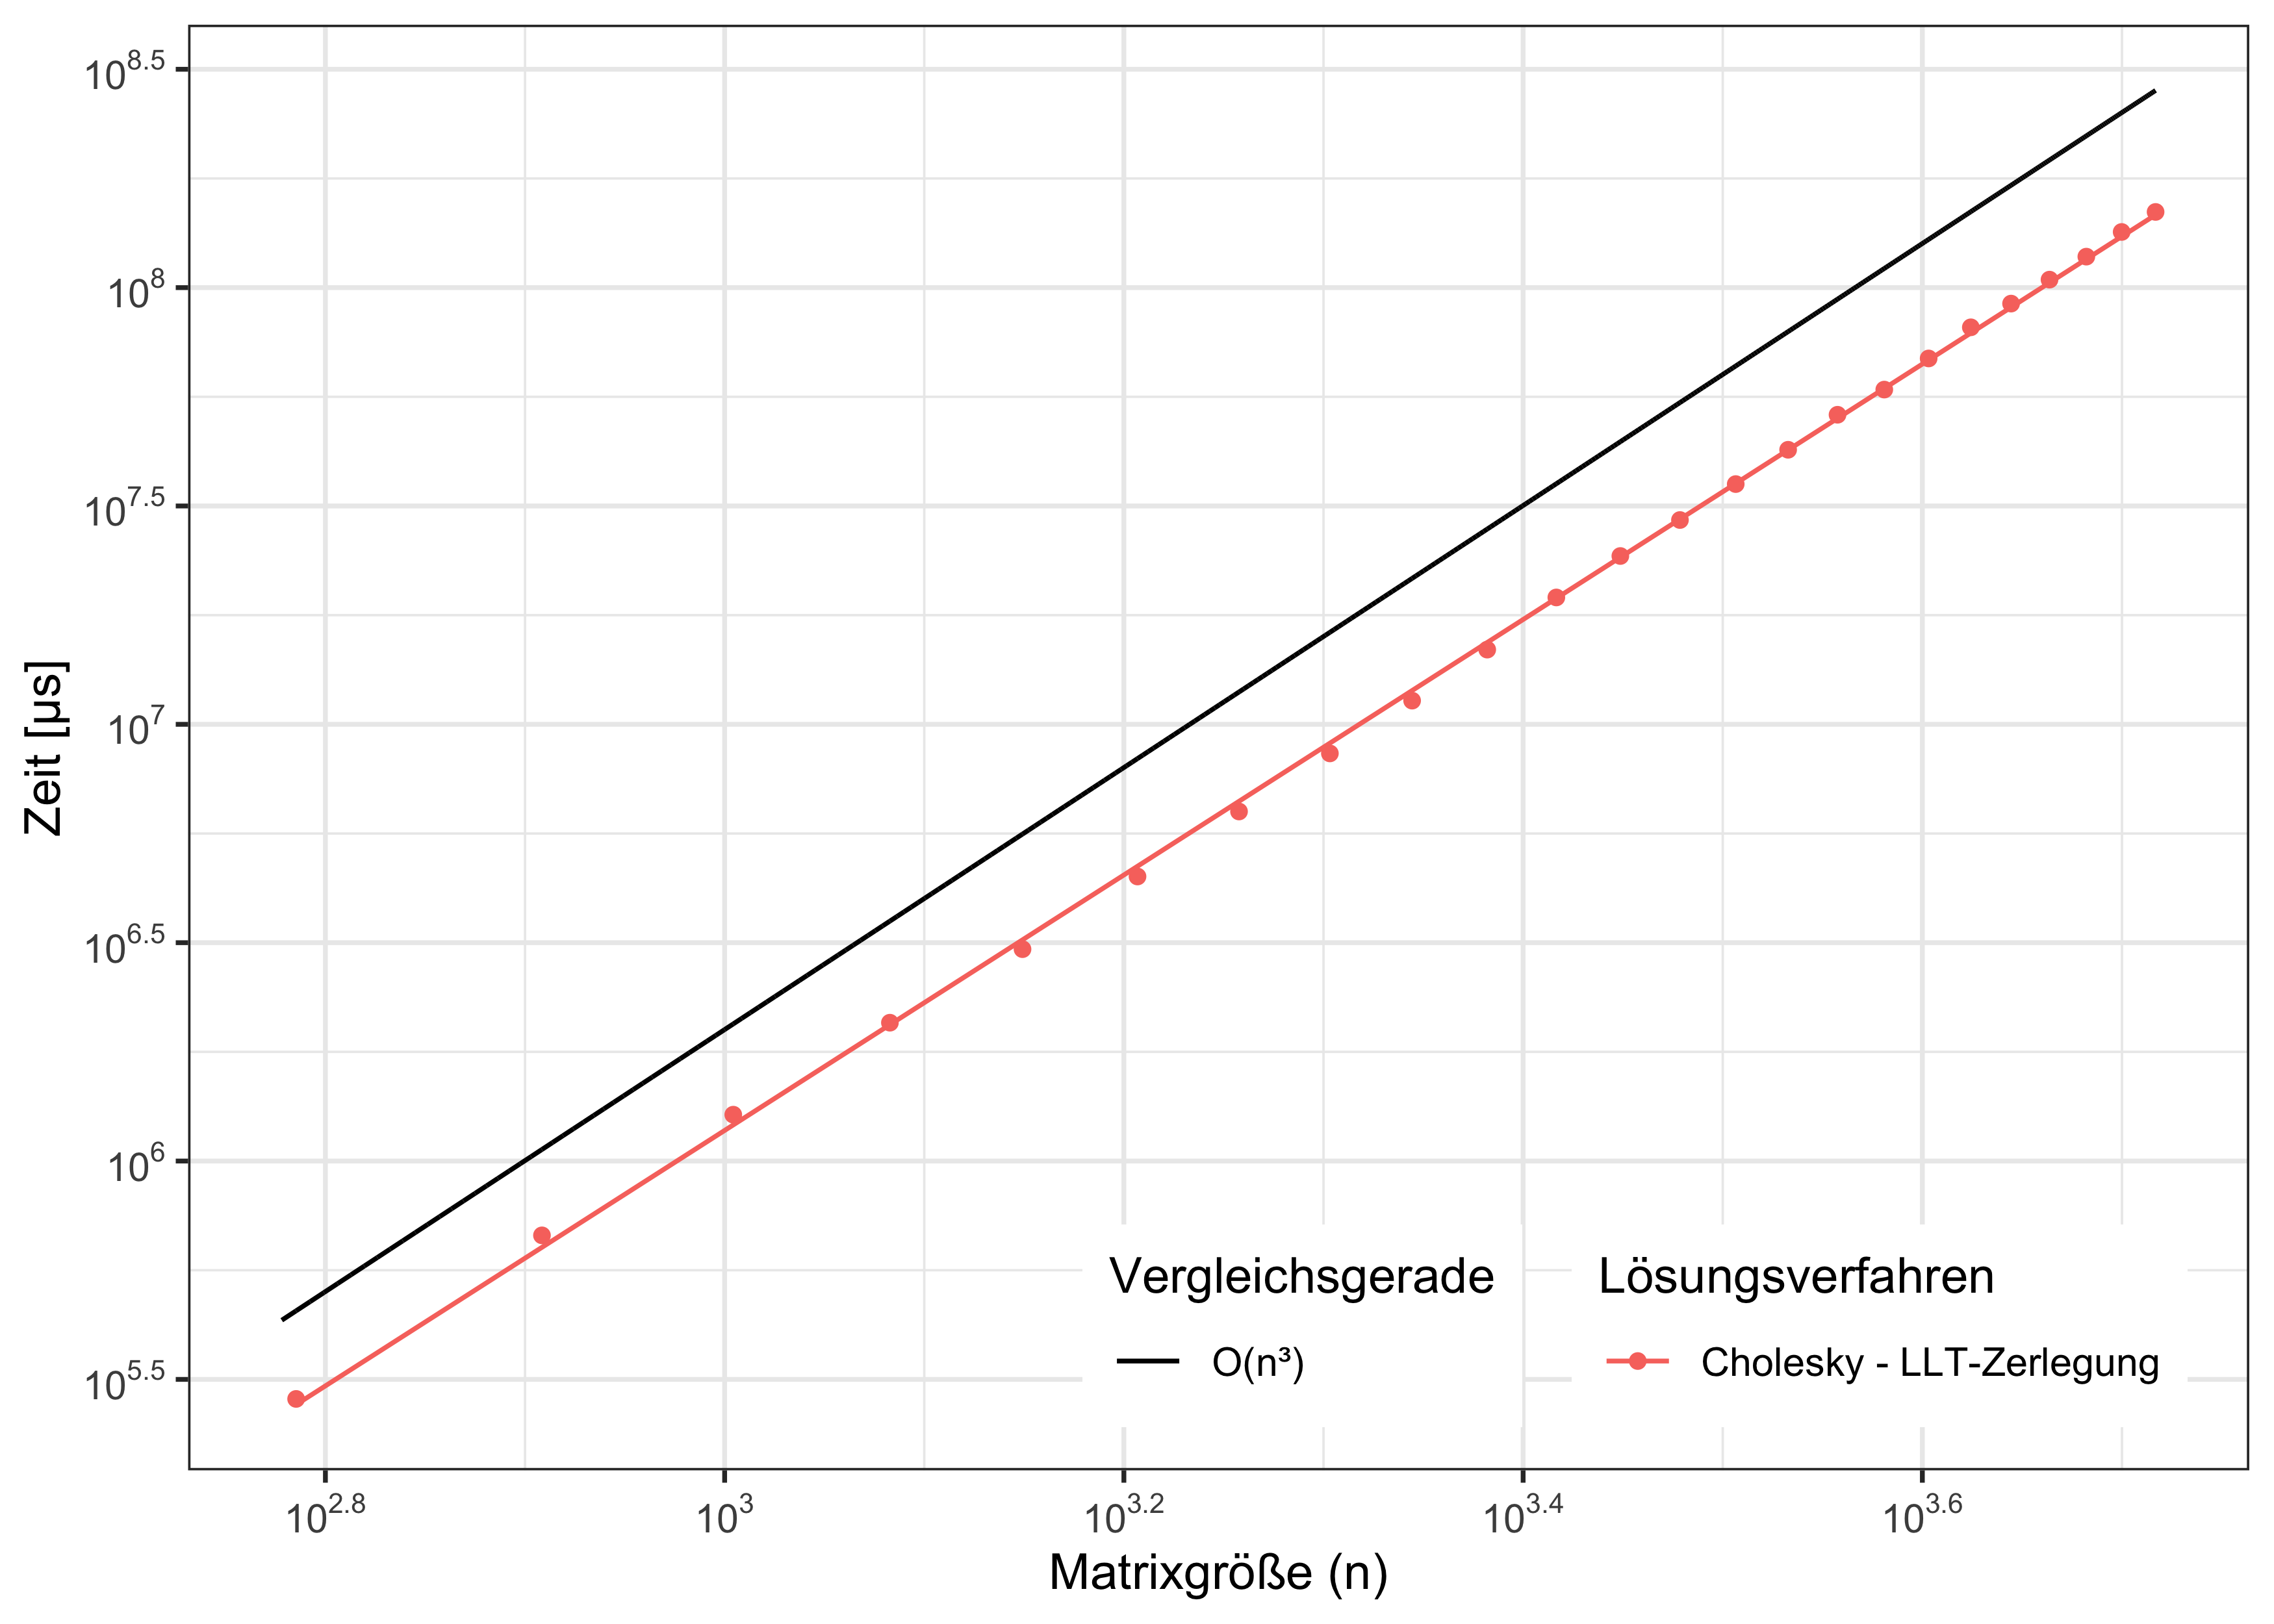
\includegraphics[width=0.8\textwidth]{../plots/eigen.png}
		\end{center}
		\caption{Ben\"otigte Zeit in $\mu s$ um Gleichungssysteme mit verschieden gro\ss en dicht besetzte $n\times n$-Koeffizientenmatrizen mittels Cholesky-Zerlegung zu l\"osen}
		\label{fig:zeiteigensolver}	
	\end{figure}
	
	\section{CG-Verfahren (Verfahren der konjugierten Gradienten)}
	
	Ist  $A\in\mathbb{R}^{n\times n}$ eine symmetrisch positiv definite Matrix dann kann die Lösung $x$ mithilfe des CG-Verfahrens beliebig genau approximiert werden.\\
	Das CG-Verfahren ist äquivalent zur Minimierung der Energiefunktion $\phi(x) = \frac{1}{2}x^{T}Ax - x^{T}b$, also $\nabla\phi(x) = Ax - b = 0$. Weil $A$ positiv definit ist, ist x ein Minimum. Man rechnet für einen zufälligen Vvektor $x_0$ das Residuum $r_0 = Ax_0 - b$ aus und nähert sich dann rekursiv der exakten Lösung $x$ an. Dabei ist nach höchstens $n$ Iterationen $\norm{x_t - x} = 0$.
	
	\begin{algorithm}[H]
		\textbf{Input:} Sei $A\in$ $\mathbb{R}^{n\times n}, b, x_0 \in \mathbb{R}^{n}$ und eine Toleranz $\tau > 0$
		\begin{algorithmic}[1]
			\State $r_0 = b - Ax_0$
			\State $d_0 = r_0$
			\State $t = 0$
			\While{$ \norm{r_t} > \tau $}
			\State $z = Ad_t$
			\State $\alpha_t = \frac{r_t^{T}r_t}{d_t^{T}z}$
			\State $x_{t+1} = x_{t} + \alpha_t d_t$
			\State $r_{t+1} = r_t - \alpha_t z$
			\State $\beta_t = \frac{r_{t+1}^{T}r_{t+1}}{r_t^{T}r_t}$
			\State $d_{t+1} = r_{t+1} + \beta_td_t$
			\State $t = t + 1$
			\EndWhile
		\end{algorithmic}
		\textbf{Output:} Näherung $x_t$ an $x = A^{-1}b$ mit $\norm{Ax_t-b} < \tau$
		
		\caption{CG-Verfahren} \label{alg:cg}
	\end{algorithm}
	
	\lstinputlisting[language=C++, firstline = 411, lastline= 439, caption = Implementierung des CG-Verfahrens in C++]{../code/Linag/densematrix.h} 
	
		
	Nun stellt sich die Frage, ob \cref{alg:cg} äquivalent zum Algorithmus 8.10 \autocite[101]{skript} ist und welcher zu bevorzugen ist.\\
	\cref{alg:cg} beinhaltet lauter Vektor-Vektor Multiplikationen und zwei Matrix-Vektor Multiplikation, es ist klar, dass die Matrix-Vektor Multiplikation aufwendiger ist als die Vektor-Vektor Multiplikation. Im Algorithmus wird die selbe Matrix-Vektor Multiplikation durchgeführt, d.h. man braucht sich nur einmal das Ergebnis auszurechnen und abzuspeichern. Beim Algorithmus 8.10 gibt es wieder zwei Matrix-Vektor Multiplikationen die die Vektor-Vektor Multiplikationen dominieren. In diesen Algorithmus müssen jedoch zwei unterschiedliche Rechnungen durchgeführt werden, und damit ist \cref{alg:cg} effizienter. Man muss nur noch zeigen, dass die beiden Algorithmen dasselbe Ergebnis liefern.\\
	Man sieht offensichtlich, dass sich die Algorithmen nur in den While-Schleifen unterscheiden. Zuerst sein in Algorithmus 8.10 angemerkt, dass man Zeile 7 am Ende der While-Schleife verschieben kann und die $t$ in Zeile 8-10 durch $t + 1$ ersetzen kann. \\
	Durch Multiplizieren von $A$ von links in Zeile 6 im Algorithmus 8.10 folgt
	\begin{align*}
		Ax_{t+1} = Ax_t + \alpha_tAd_t
	\end{align*} 
	und somit
	\begin{align}\label{r}
		r_{t+1} = b - Ax_{t+1} = b - Ax_t - \alpha_tAd_t = r_t - \alpha_tAd_t
	\end{align}
	
	\cref{r} kann man umformen in 
	\begin{align*}
		r_{t+1} =  r_t - \alpha_tAd_t \Leftrightarrow Ad_t = \frac{1}{\alpha_t}(r_t - r_{t+1})
	\end{align*}
	Das heißt der Zähler von $\beta_t$ kann folgendermaßen umgeschrieben werden
	\begin{align*}
		r_{t+1}^{T}Ad_t = \frac{1}{\alpha_t}r_{t+1}^{T}(r_t - r_{t+1}) = -\frac{1}{\alpha_t}r_{t+1}^{T}r_{t+1}
	\end{align*}
	da die Residieen orthogonal sind und der Nenner
	\begin{align*}
		d_t^{T}Ad_t = (r_t + \beta_{t-1}d_{t-1})^{T}Ad_t =  \frac{1}{\alpha_t}r_{t}^{T}(r_t - r_{t+1}) = \frac{1}{\alpha_t}r_t^{T}r_t 
	\end{align*}
	da die Suchrichtungen $d_t$ $A$-orthogonal sind.
	Also folgt insgesamt
	\begin{align*}
		\beta_t = -\frac{r_{t+1}^{T}Ad_t}{d_t^{T}Ad_t} = -\frac{-\frac{1}{\alpha_t}r_{t+1}^{T}r_{t+1}}{\frac{1}{\alpha_t}r_t^{T}r_t } = \frac{r_{t+1}^{T}r_{t+1}}{r_t^{T}r_t }
	\end{align*}
	Außerdem folgt durch einsetzen von Zeile 10 in Zeile 5
	\begin{align*}
		\alpha_t = \frac{r_t^{T}d_t}{d_t^{T}Ad_t} = \frac{r_t^{T}(r_t + \beta_{t-1}d_t)}{d_t^{T}Ad_t} = \frac{r_t^{T}r_t}{d_t^{T}Ad_t}
	\end{align*}
	da \autocite[vgl.][100]{skript}
	\begin{align*}
		r_t^{T}d_j = 0 \quad \forall \text{ }0 \leq j < t
	\end{align*}
	
	
	
	
	Für die Iteration des CG-Verfahrens (ohne Abbruchkriterium) gilt die Fehlerabschätzung \autocite[vgl.][102]{skript}
	\begin{align*}
		\norm{x^{(t)} - A^{-1}b}_A \leq 2\left(\frac{\sqrt{\kappa} - 1}{\sqrt{\kappa} + 1}\right)^{t}\norm{x^{(0)} - A^{-1}b}_A, \quad t\in\mathbb{N}
	\end{align*}
	
	mit der spektralen Konditionszahl der Matrix $\kappa(A) := \left|\frac{\lambda_{max}(A)}{\lambda_{min}(A)}\right|$ und der Energienorm $\norm{x}_A := \sqrt{(x,x)_A}$. Das Verfahren konvergiert für $\frac{\sqrt{\kappa} - 1}{\sqrt{\kappa} + 1} < 1$, was offensichtlich gegeben ist, da $\kappa \geq 1$. Die Konvergenzgeschwindigkeit ist größer, wenn der Bruch minimal ist, also genau dann wenn die Eigenwerte der Matrix eng zusammenliegen. Wenn alle Eigenwerte gleich sind, dann gilt $\kappa = 1$ also $\frac{\sqrt{\kappa} - 1}{\sqrt{\kappa} + 1} = 0$. 
	
	\subsection{Dünn besetzte Matrizen}
	
	Da man beim lösen linearer Gleichungssysteme oft mit großen, dünn besetzten Matrizen arbeitet, ist es sinnvoll nur Einträge ungleich Null zu speichern. Dafür kann zum Beispiel das sogenannte \textit{"compressed spare row"} Format verwendet werden. Bei der Implementierung dieses Formats werden anstelle aller Einträge $A_{i,j}, i,j = 1,\ldots,n$ einer Matrix $A\in$ $\mathbb{R}^{n\times n}$ ein Vektor $v\in\mathbb{R}^{m}$ aller Einträge ungleich Null, ein Vektor $J\in\mathbb{N}_0^{m}$ von Spaltenindizes und ein Vektor $I\in\mathbb{N}_0^{n+1}$ gespeichert.
	
	Die $i-$te Zeile von A ist gegeben durch
	\begin{align*}
		A_{i,j} = 
		\begin{cases}
			\textit{$v_{k(j)}$},&\quad\textit{falls $j \in \{J_{I_i}, J_{I_{i}} + 1, \ldots, J_{I_{i+1}} - 1$}\}\\
			\textit{0},&\quad\textit{sonst}\\
		\end{cases}
	\end{align*} 
	wobei $J_{k_{(j)}} = j$.\\
	
	Eine Möglichkeit das Format zu implementieren ist wie folgt:
	
	\lstinputlisting[language=C++, firstline = 170, lastline= 204, caption = Speicherung einer Matrix im compressed spare row Format]{../code/Linag/sparsematrix.h} 
	
	\lstinputlisting[language=C++, firstline = 536, lastline= 552, caption = compressed spare row Format zu densematrix]{../code/Linag/densematrix.h} 
	
	

	In \cref{fig:zeitcg-sparse} ist zu sehen, dass das CG-Verfahren f\"ur d\"unn besetzte Matrizen im \textit{compressed sparse row}-Format wesentlich effizienter berechnet werden kann, als f\"ur vollbesetzte Matrizen bzw. als solche gespeicherten Matrizen.
	Wie in Zeile 5 in \cref{alg:cg} zu sehen ist, ist der unterschiedliche Aufwand von einer Matrix-Vektor-Multiplikation abh\"angig. Der Aufwand um eine vollbesetzte $n\times n$-Matrix mit einem Vektor zu multiplizieren entspricht $\mathcal{O}(n^2)$. Der Aufwand um eine d\"unnbesetzte Matrix mit einem Vektor zu multiplizieren ist mit $\mathcal{O}(n)$ linear und davon abh\"angig wie dicht die Matrix besetzt ist. Außerdem ist zu sehen, wie sich die ben\"otigte Zeit zur durchf\"uhrung des CG-Verfahrens mit der Anzahl an Eintr\"agen ungleich null pro Zeile der Matrix \"andert.
	
	\begin{figure}[H]
		\begin{center}
			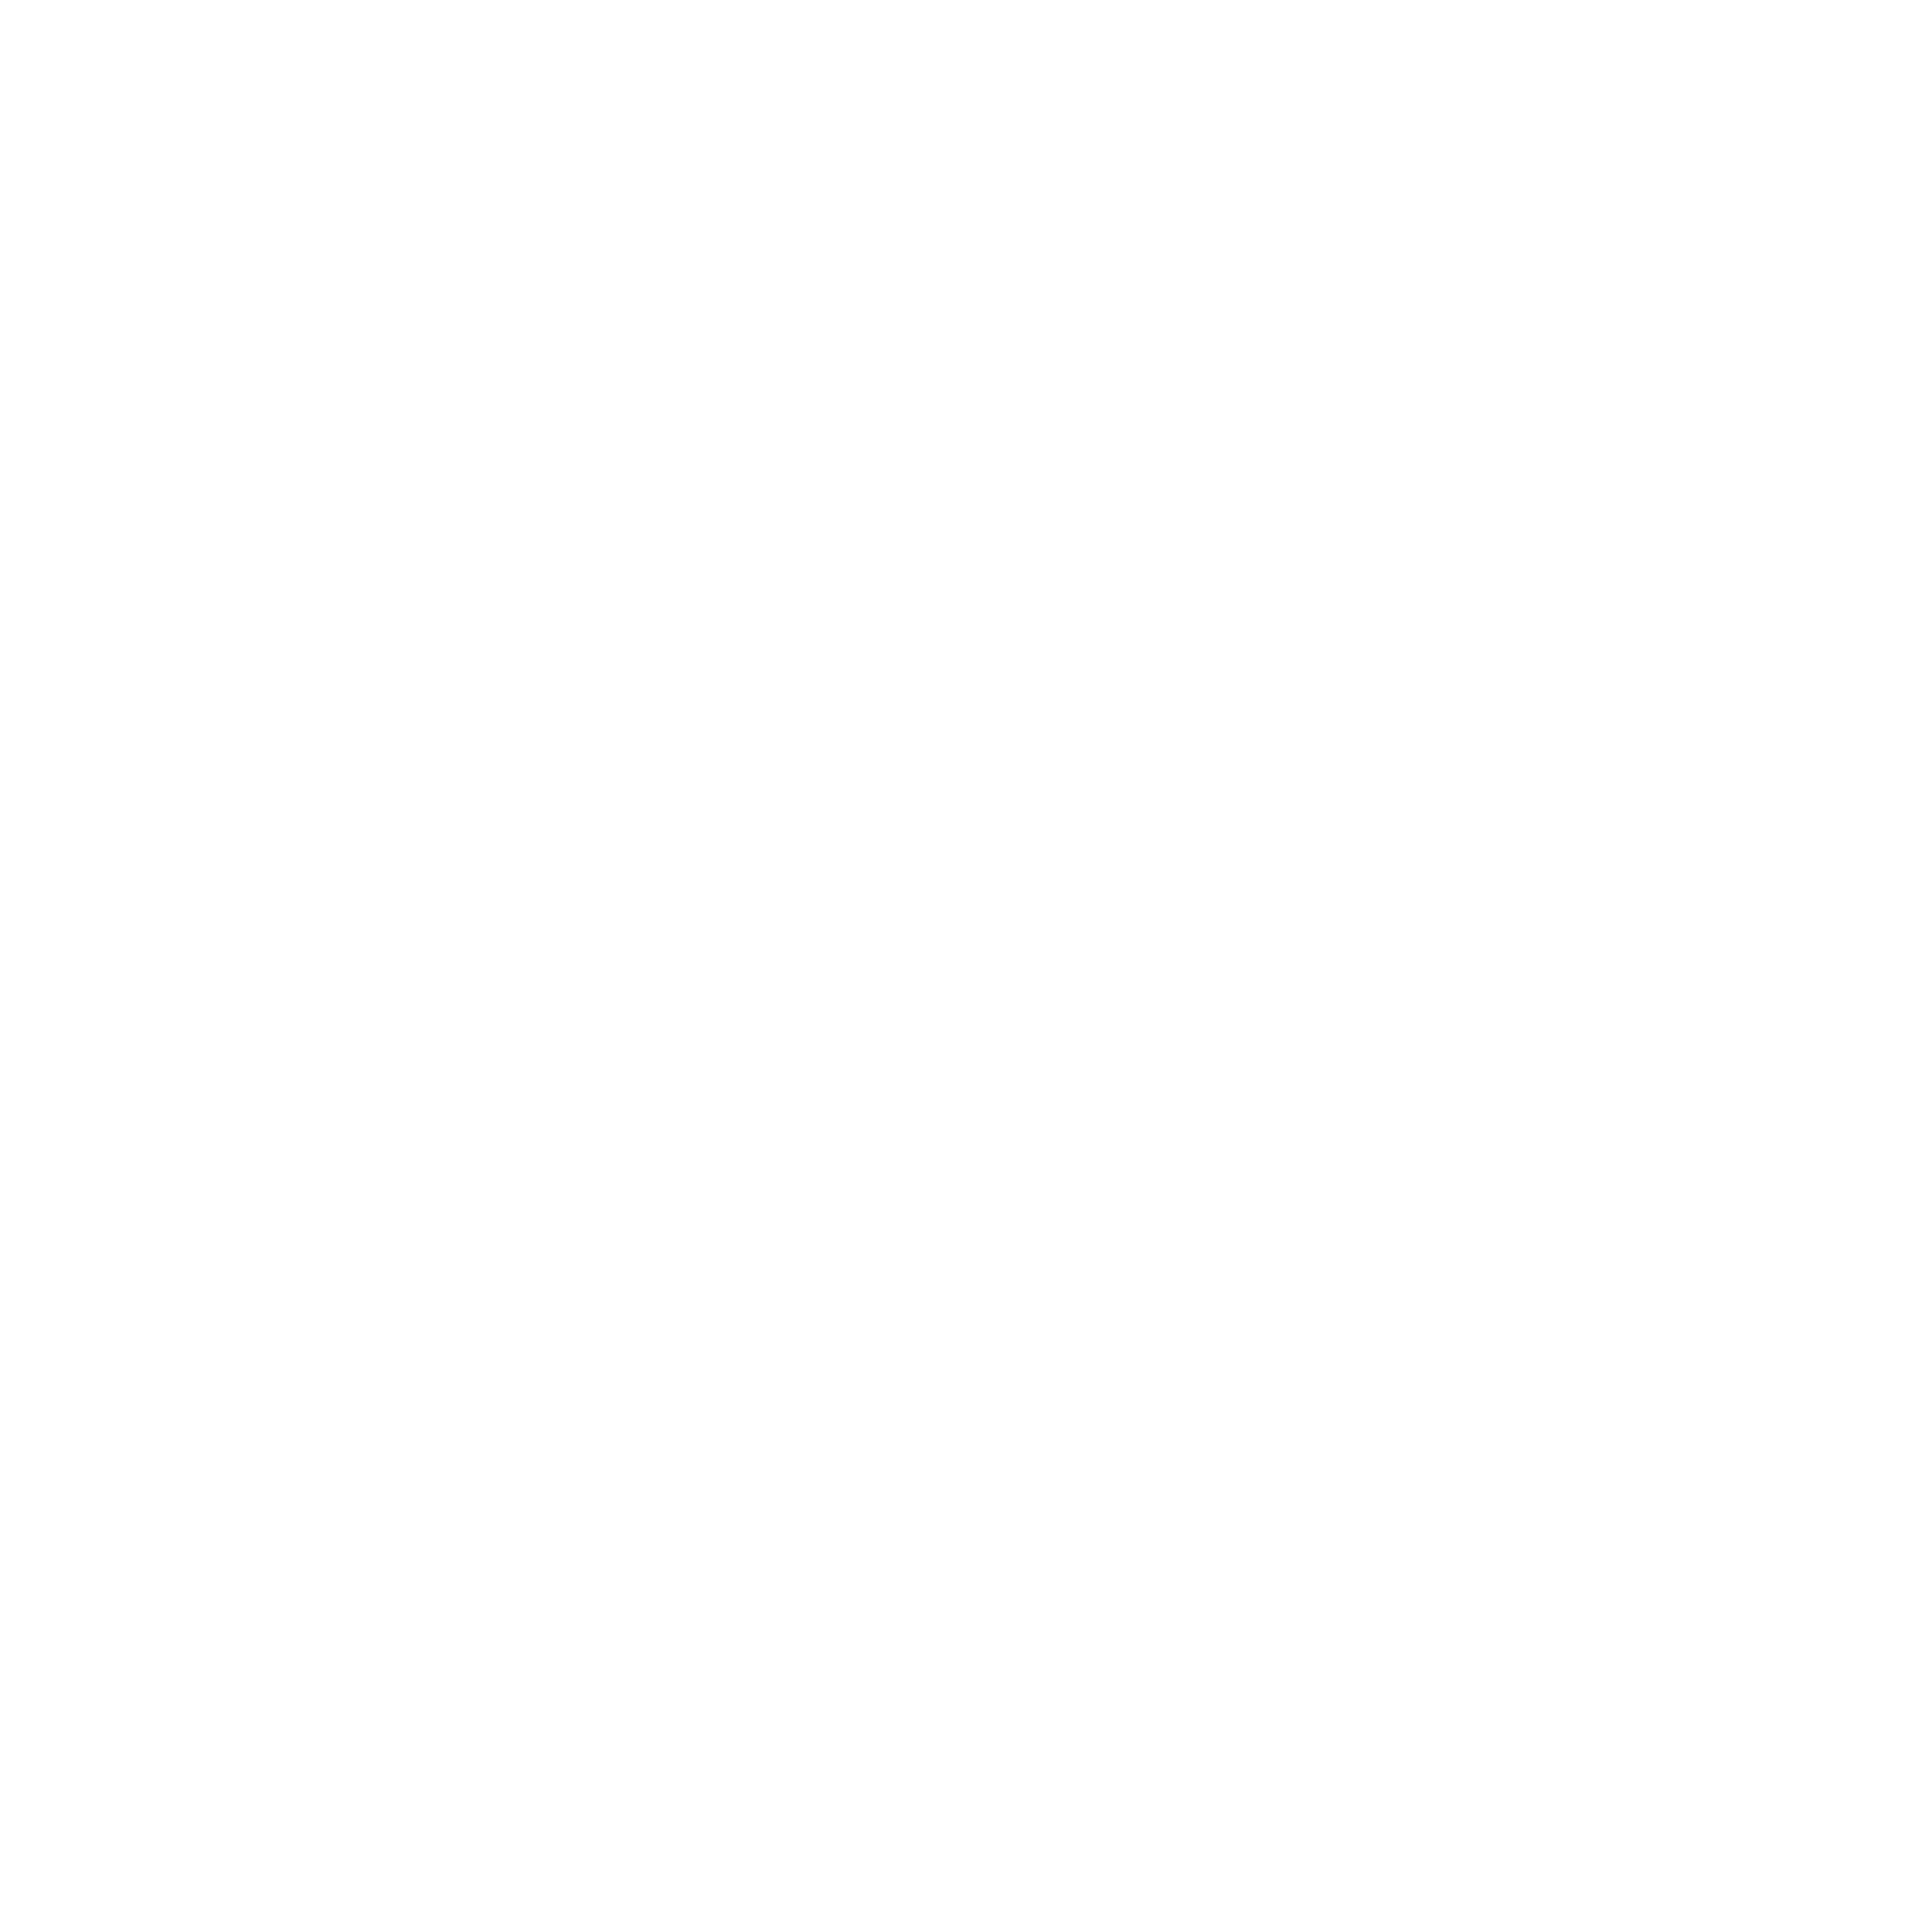
\includegraphics[width=0.8\textwidth]{../plots/cg-sparsity-sparse.png}
		\end{center}
		\caption{Ben\"otigte Zeit in $\mu s$ f\"ur verschieden dicht besetzte $n\times n$-Matrizen im \textit{compressed sparse row}-Format}
		\label{fig:zeitcg-sparse}	
	\end{figure}
	
	\subsection{Vorkonditionierung}
	Die spektrale Konditionszahl definiert die Konvergenzgeschwindigkeit des CG-Verfahrens. Durch lösen des vorkonditionierten Systems
	\begin{align*}
		D^{-1}AD^{-T}y = D^{-1}b
	\end{align*}
	kann die Konvergenz beschleunigt werden und man bekommt eine Lösung x der Form 
	\begin{align*}
		x = D^{-T}y
	\end{align*}
	Man wählt die Matrix D so, dass für beliebige $z \in \mathbb{R}^{n}$ der Vektor $D^{-T}D^{-1}z$ einfach zu berechnen ist und zugleich $cond(D^{-1}AD^{-T}) < cond(A)$ gilt. Das heißt mithilfe der Matrix $D$ liegen die Eigenwerte enger zusammen und die spektrale Konditionszahl wird kleiner. 
	\begin{algorithm}[H]
		\textbf{Input:} Sei A$\in$ $\mathbb{R}^{n\times n}, x_0 \in \mathbb{R}^{n}, P:=DD^{T}$ und eine Toleranz $\tau > 0$
		\begin{algorithmic}[1]
			\State $r_0 = b - Ax_0$
			\State $z_0 = P^{-1}r_0$
			\State $d_0 = z_0$
			\State $t = 0$
			\While{$ \norm{r_t} > \tau $}
			\State $z = Ad_t$
			\State $\alpha_t = \frac{r_t^{T}z_t}{d_t^{T}z}$
			\State $x_{t+1} = x_{t} + \alpha_t d_t$
			\State $r_{t+1} = r_t - \alpha_t z$
			\State $z_{t+1} = P^{-1}r_{t+1}$
			\State $\beta_t = \frac{z_{t+1}^{T}r_{t+1}}{z_tr_t}$
			\State $d_{t+1} = z_{t+1} + \beta_td_t$
			\State $t = t + 1$
			\EndWhile
		\end{algorithmic}
		\textbf{Output:} Näherung $x_t$ an $x = A^{-1}b$ mit $\norm{Ax_t-b} < \tau$
		
		\caption{Vorkonditionierte CG-Verfahren} \label{alg:vcg}
	\end{algorithm}

	Im Gegensatz zu \cref{alg:cg}  sind in \cref{alg:vcg} pro Iteration zwei Matrix-Vektormultiplikationen notwendig. F\"ur d\"unnbesetzte Matrizen bleibt der Aufwand mit $\mathcal{O}(n)$ also linear, wird jedoch, um eine  von der Koeffizientenmatrix abh\"angige multiplikative Konstante gr\"o\ss er. Die f\"ur einen Iterationsschritt ben\"otigte Zeit ist zusammen mit einer Vergleichsgerade f\"ur $\mathcal{O}(n)$ in \cref{fig:precond-vs-cg-complexity} zu sehen. 
	
	\begin{figure}[H]
		\begin{center}
			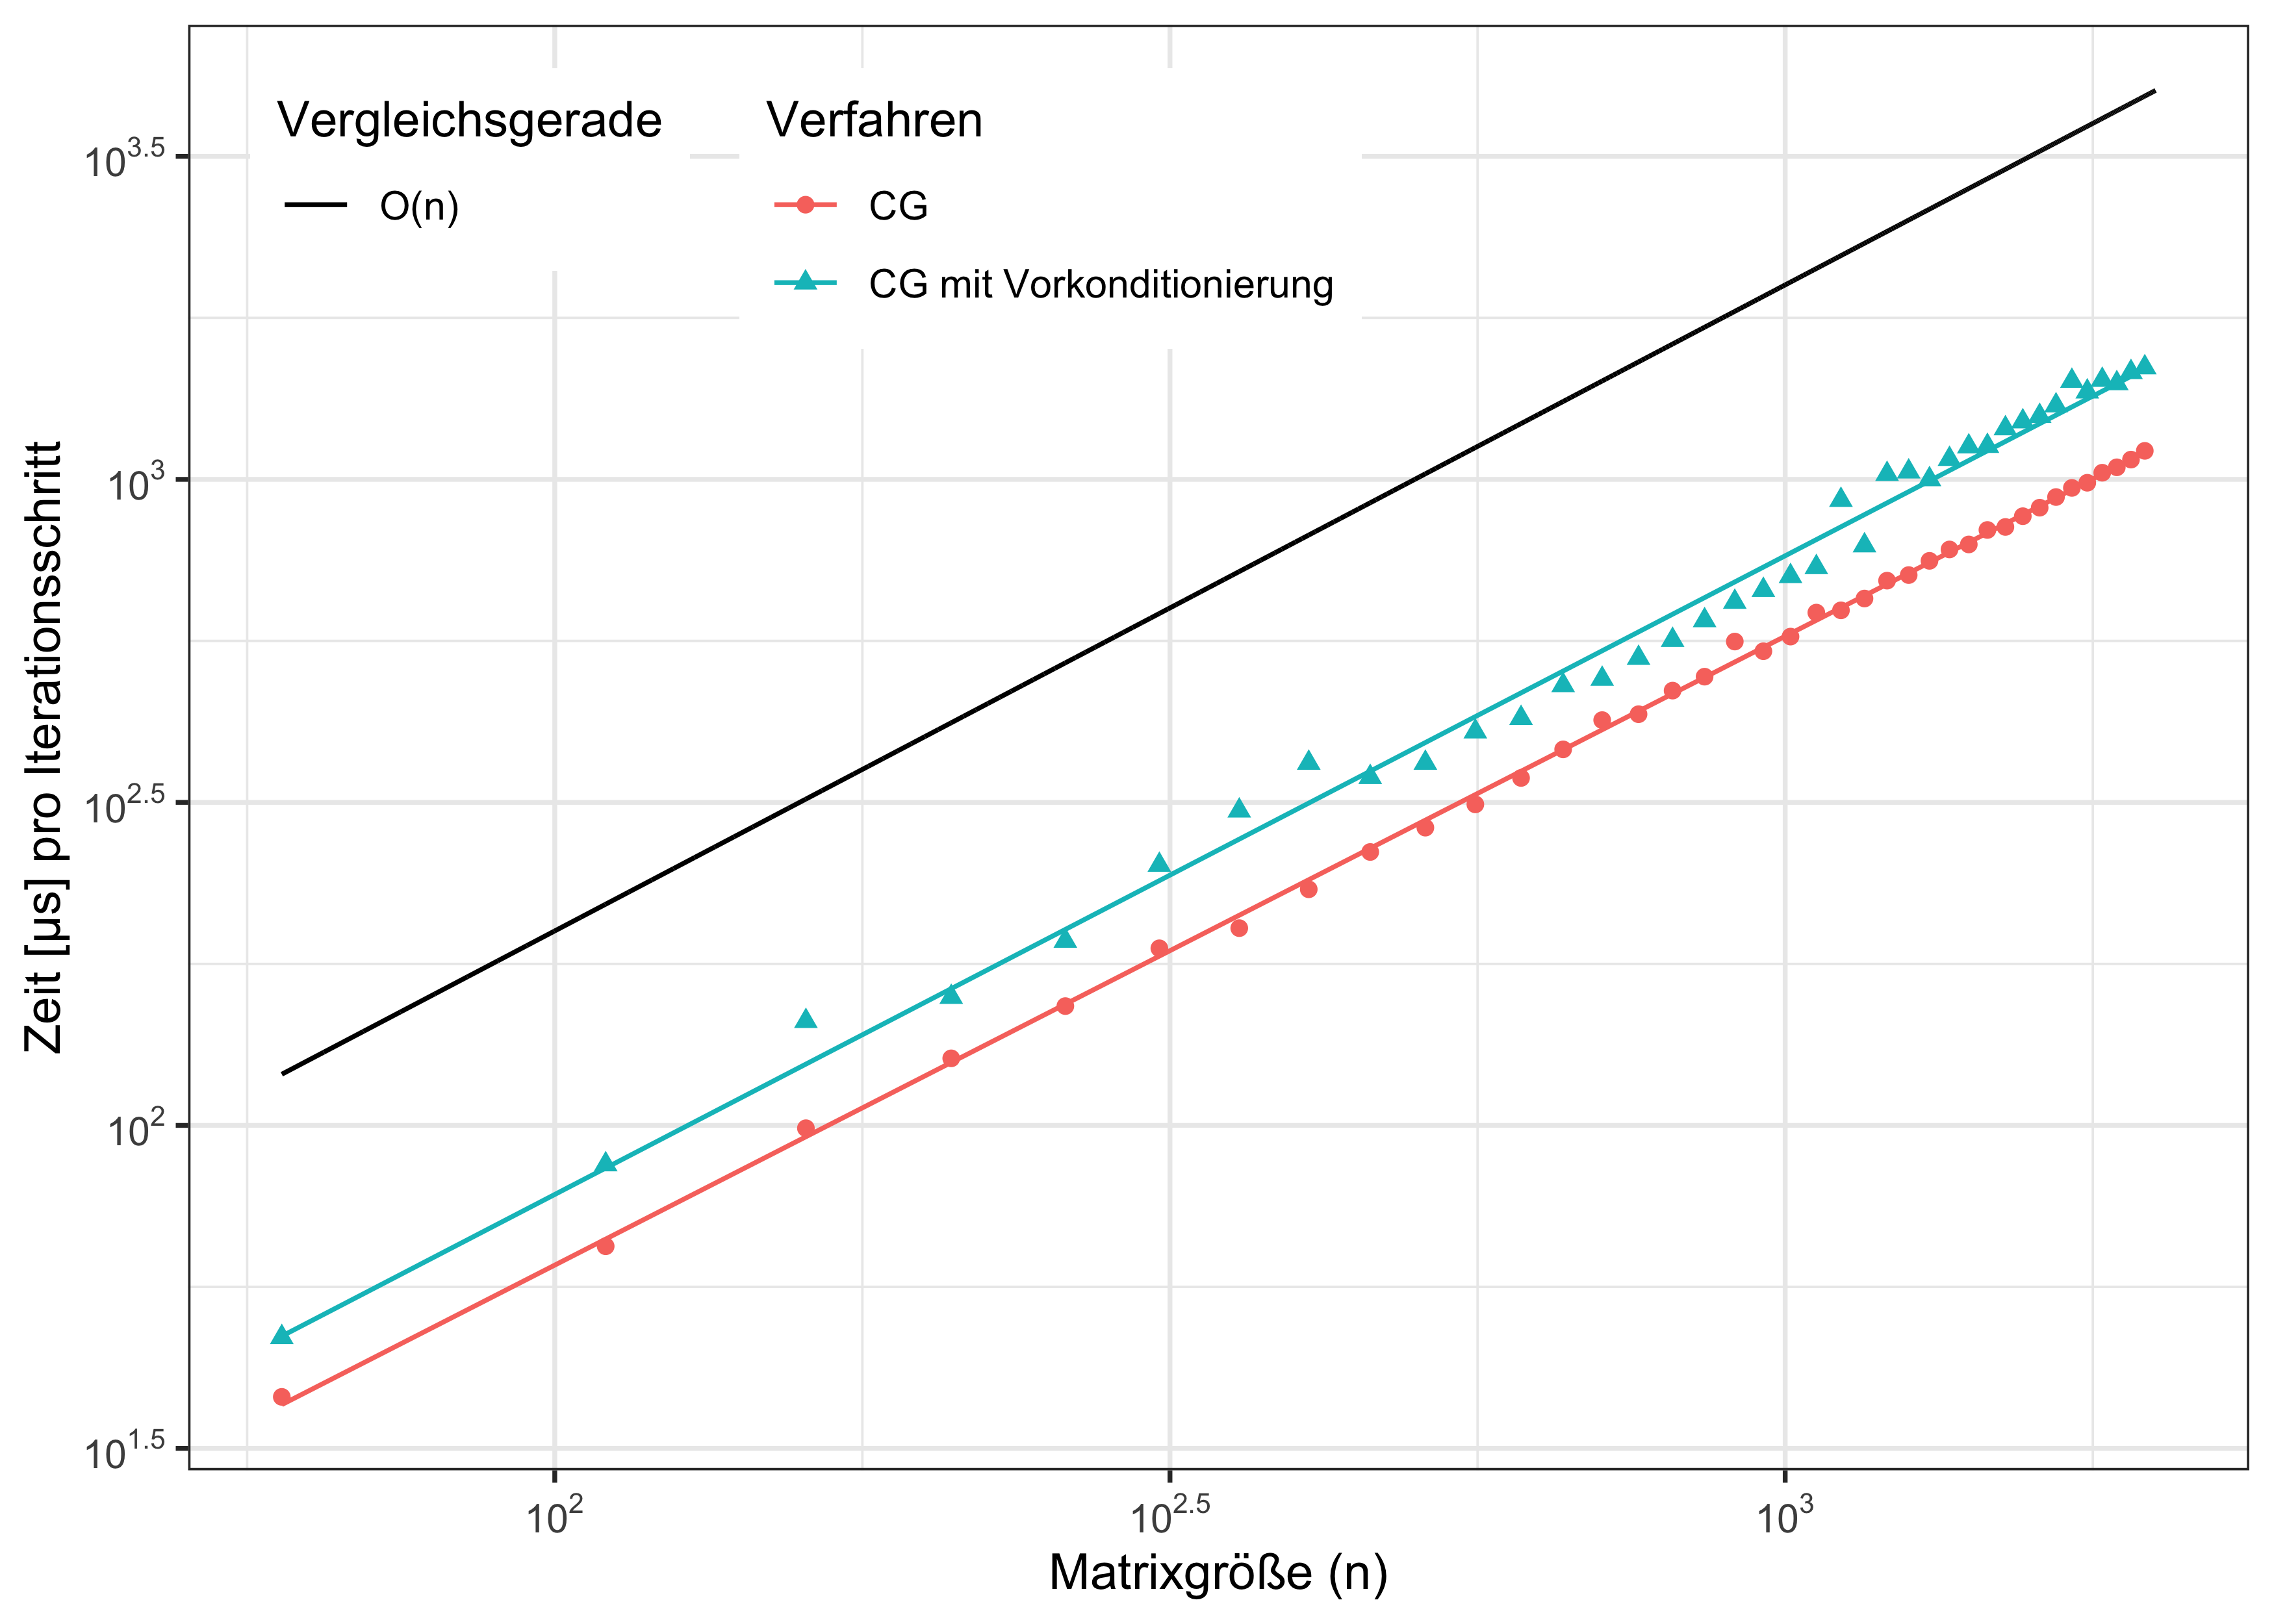
\includegraphics[width=0.8\textwidth]{../plots/precond-vs-cg-complexity.png}
		\end{center}
		\caption{Residuum nach Iterationsschritt $t$ f\"ur vorkonditioniertes CG- und CG-Verfahren }
		\label{fig:precond-vs-cg-complexity}	
	\end{figure}
	
	In \cref{fig:precond-vs-cg} ist zu sehen, dass aufgrund der kleineren Konditionszahl wesentlich weniger Iterationsschritte benötigt werden, bzw. das vorkonditionierte CG-Verfahren, mit $P = diag(A_{11}, \ldots, A_{nn})$ schneller konvergiert. 
		
	\begin{figure}[H]
		\begin{center}
			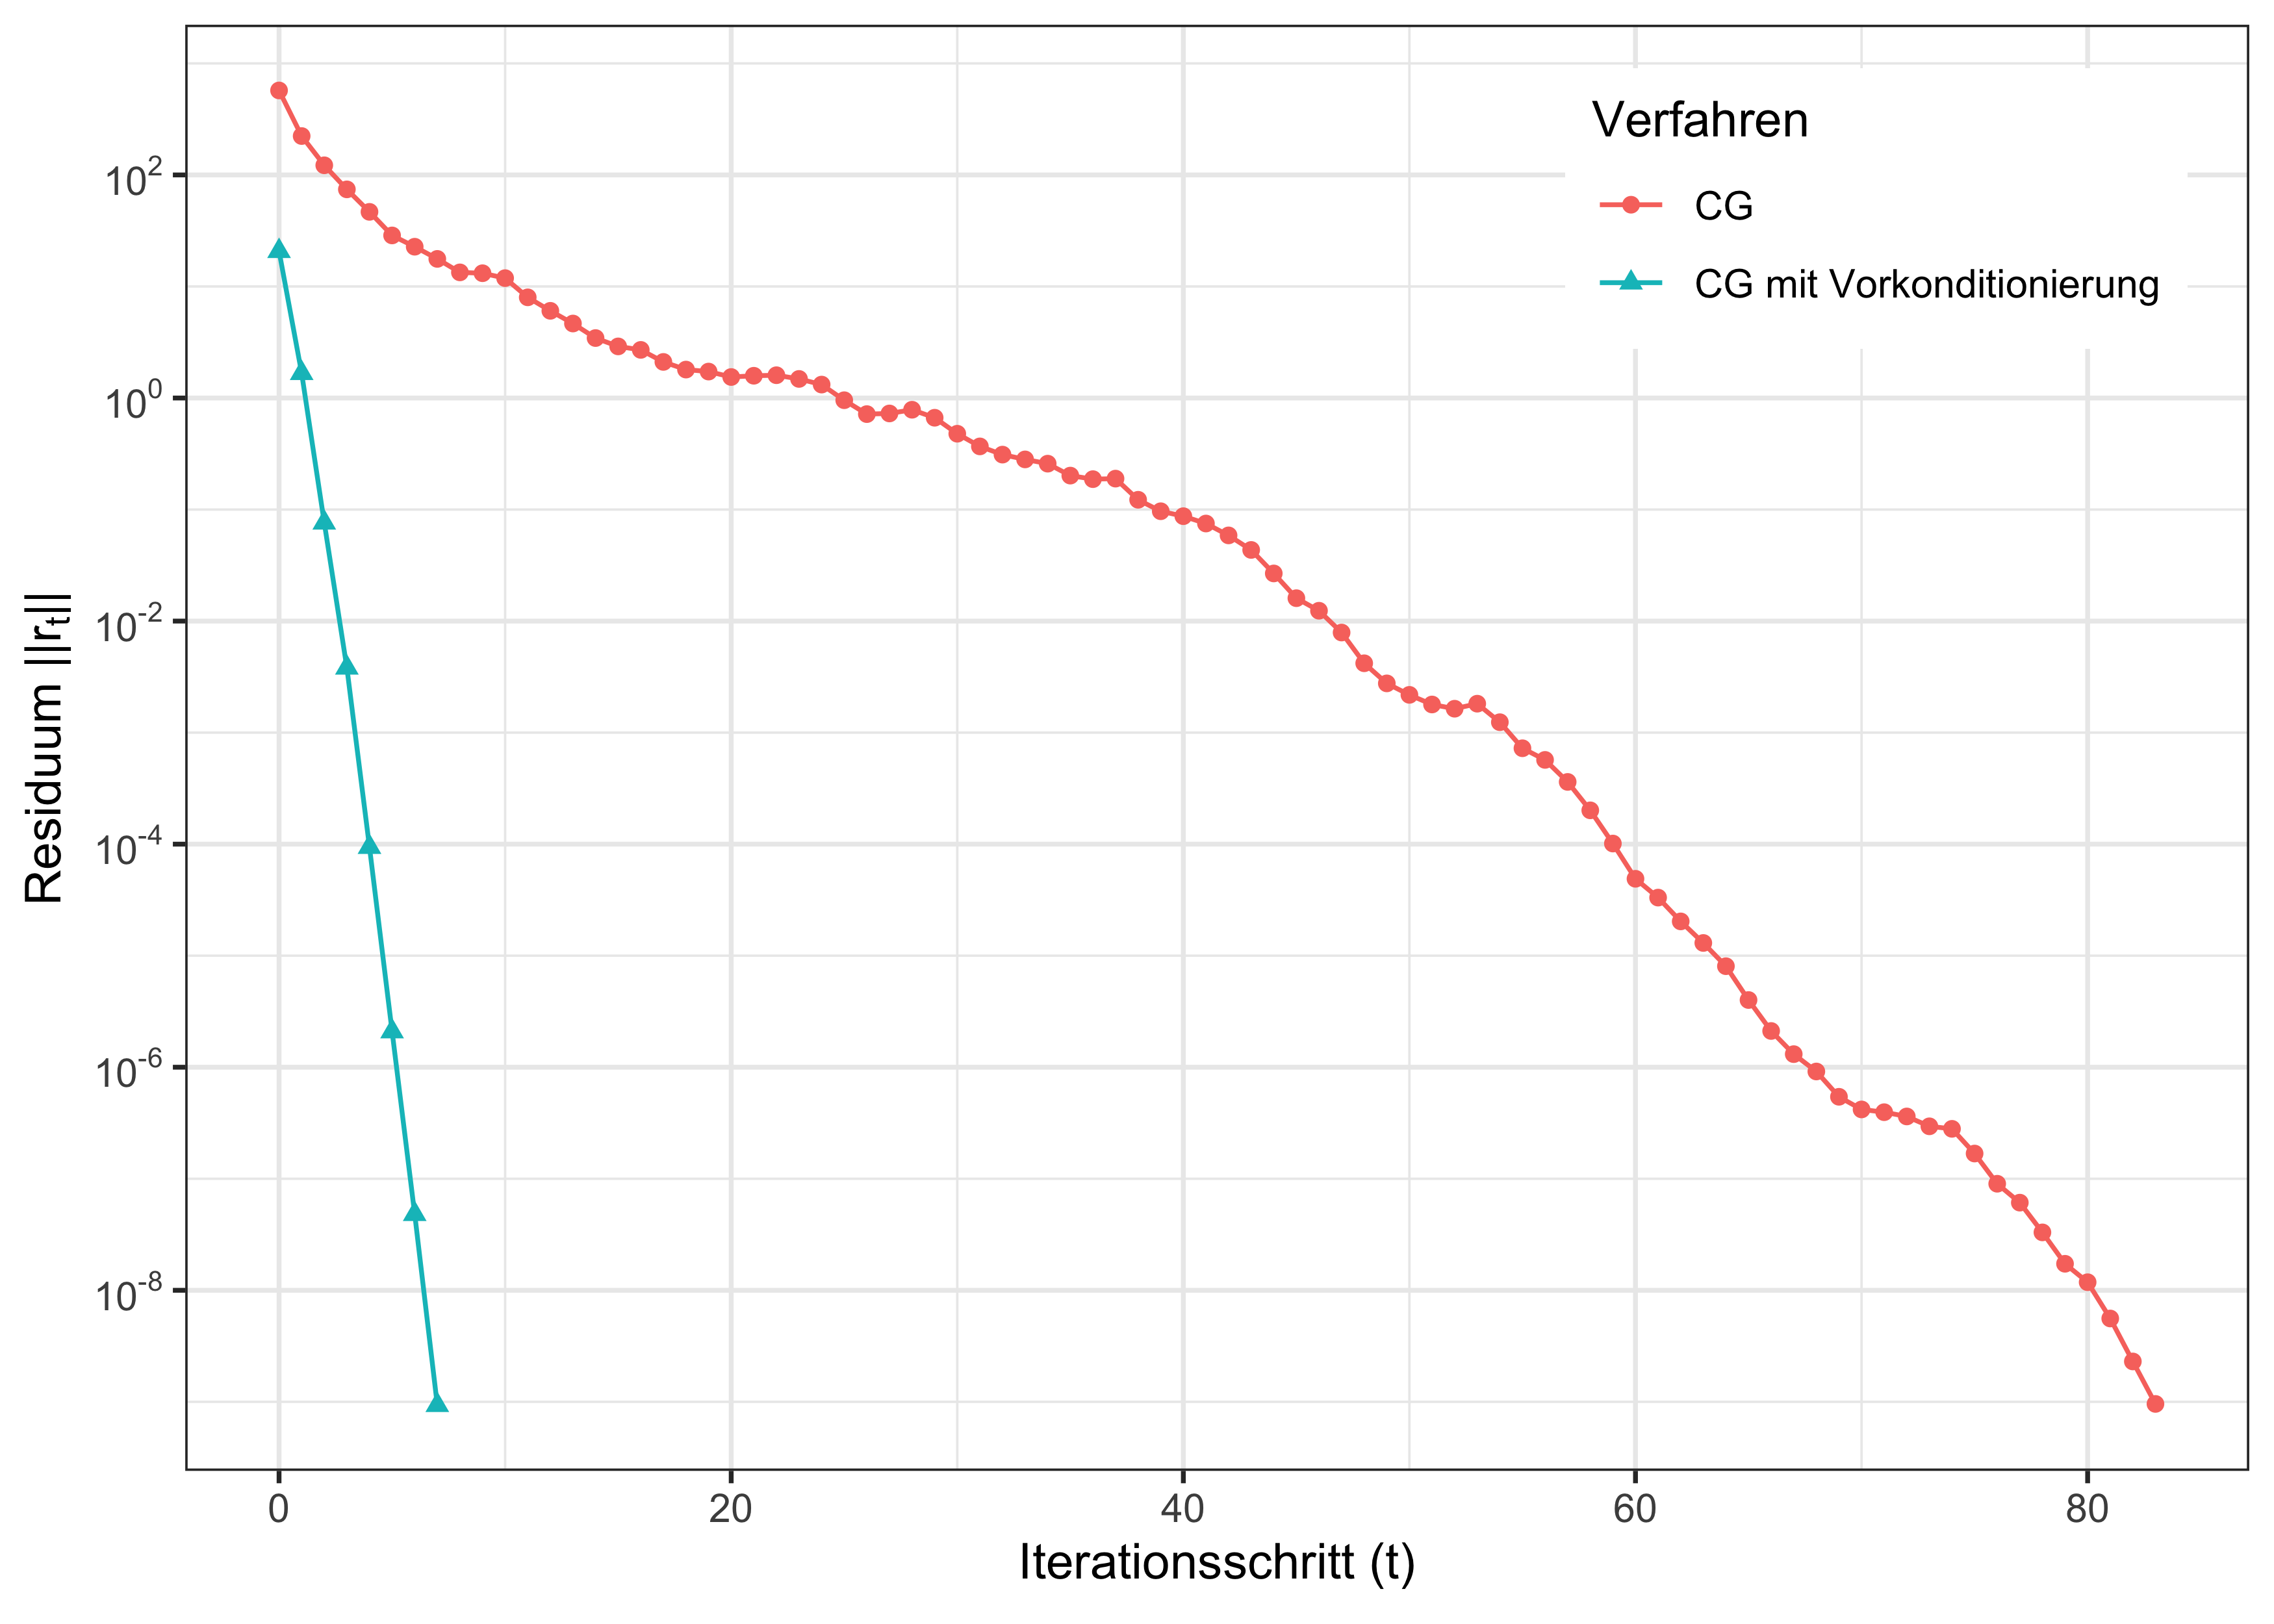
\includegraphics[width=0.8\textwidth]{../plots/precond-vs-cg.png}
		\end{center}
		\caption{Residuum nach Iterationsschritt $t$ f\"ur vorkonditioniertes CG- und CG-Verfahren }
		\label{fig:precond-vs-cg}	
	\end{figure}
	
	\newpage
	\appendix
	\section{Verwendete Klassen}
	\subsection{Size}
	\lstinputlisting[language=c,  caption=size.h]{../code/Linag/size.h}
	\subsection{Vektor}
	\lstinputlisting[language=c,  caption=vector.h]{../code/Linag/vector.h}
	\subsection{Vollbesetzte Matrix}
	\lstinputlisting[language=c,  caption=densematrix.h]{../code/Linag/densematrix.h}
	\subsection{D\"unnbesetzte Matrix}
	\lstinputlisting[language=c,  caption=sparsematrix.h]{../code/Linag/sparsematrix.h}
	
	\newpage
	\printbibliography
	\lstlistoflistings
	\listoffigures
	\thispagestyle{firststyle}
	
\end{document}

